\documentclass{beamer}

\usepackage{graphicx}
\usepackage[style=ieee]{biblatex}
\usepackage{hyperref}
\usepackage{listings}
\usepackage{xcolor}

\definecolor{codegreen}{rgb}{0,0.6,0}
\definecolor{codegray}{rgb}{0.5,0.5,0.5}
\definecolor{codepurple}{rgb}{0.58,0,0.82}
\definecolor{backcolour}{rgb}{0.95,0.95,0.92}

\lstdefinestyle{mystyle}{
    backgroundcolor=\color{backcolour},
    commentstyle=\color{codegreen},
    keywordstyle=\color{magenta},
    numberstyle=\tiny\color{codegray},
    stringstyle=\color{codepurple},
    basicstyle=\ttfamily\footnotesize,
    breakatwhitespace=false,
    breaklines=true,
    captionpos=b,
    keepspaces=true,
    numbers=left,
    numbersep=5pt,
    showspaces=false,
    showstringspaces=false,
    showtabs=false,
    tabsize=2
}

\lstset{style=mystyle}

\usetheme{Berlin}

\addbibresource{ref.bib}

\title{SciEcon Insights: Publication Guideline - GitHub}
\author{Crinstaniev}
\logo{
	
\includegraphics[width=.2\textwidth]{img/sciecon.png}
}

\begin{document}

\maketitle

\begin{frame}

	\frametitle{Table of Contents}
	\tableofcontents

\end{frame}

\section{Download}
\begin{frame}
	
	\frametitle{Download Template from GitHub}
	
	\begin{enumerate}
		\item Download the template \texttt{template.md} file from GitHub.\\ 
		Link: \url{https://github.com/SciEcon/publication-github-guideline/blob/main/template.md}
	\item Use any text editor to modify \texttt{template.md}. We highly recommend you to use \texttt{Visual Studio Code} \cite{noauthor_visual_nodate}.
	\end{enumerate}
\end{frame}

\section{Editing}

\begin{frame}
\frametitle{Edit Using VSCode}
\begin{figure}[!htbp]
	\centering
	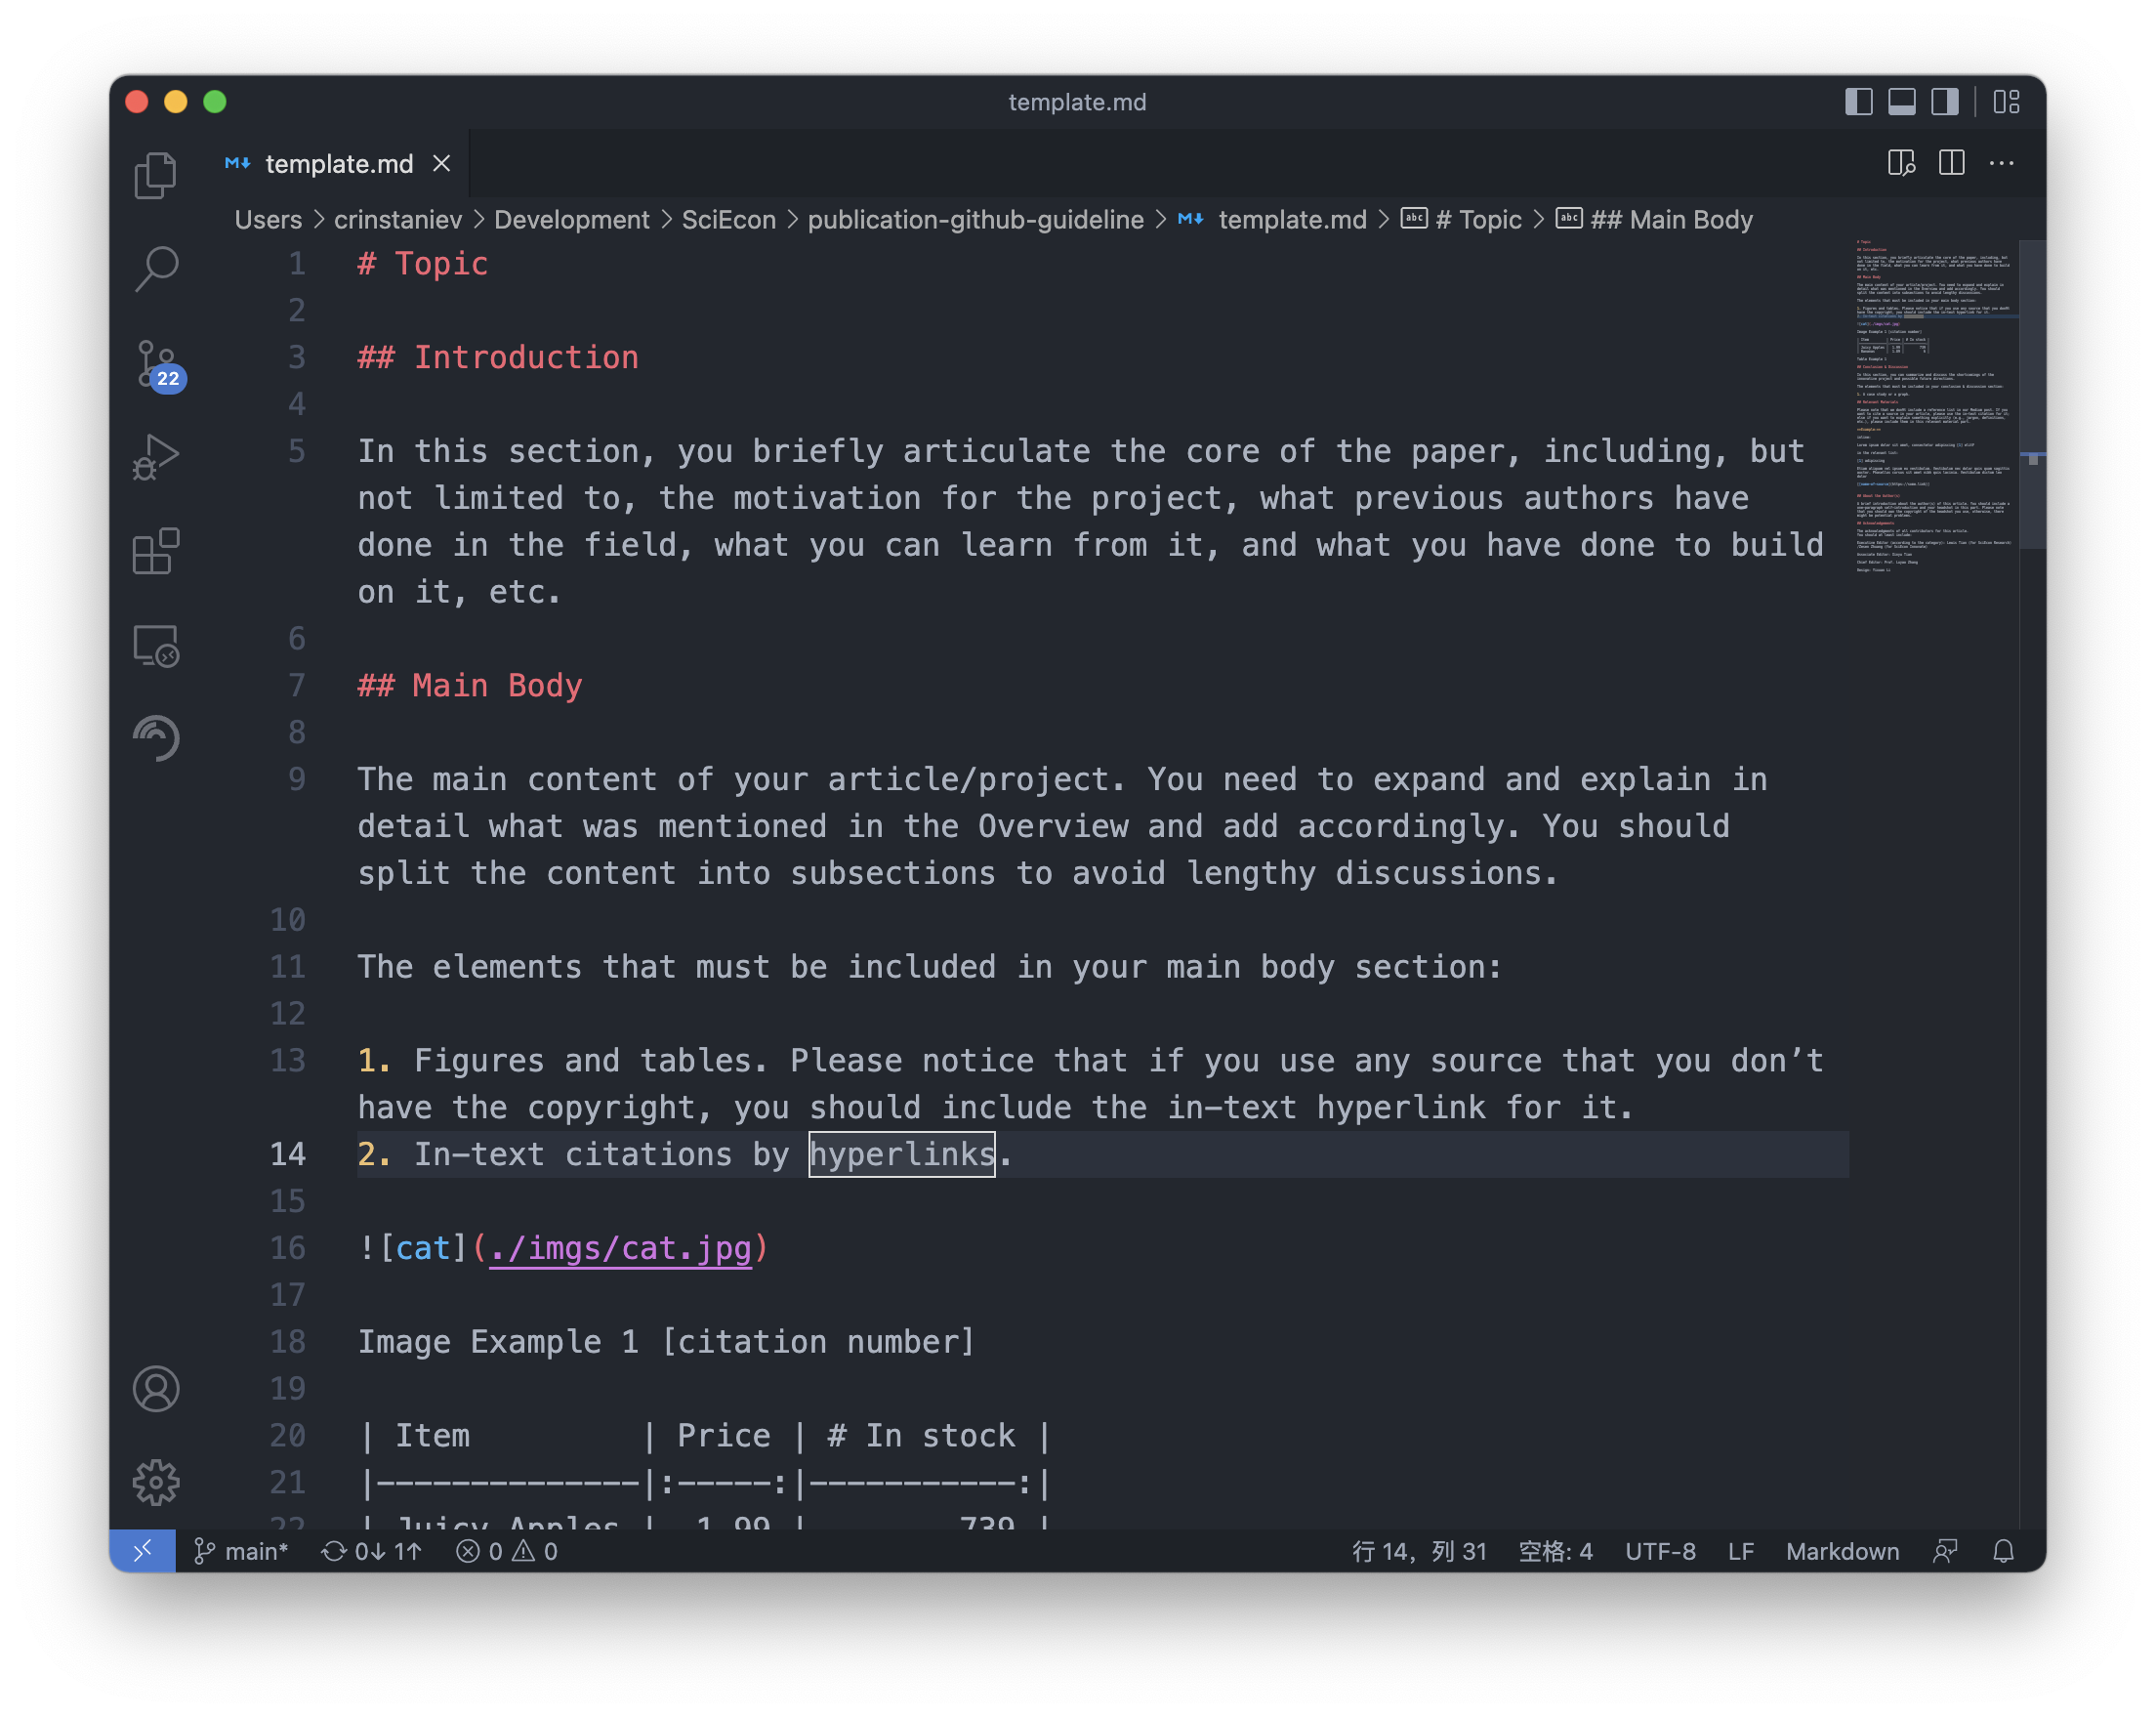
\includegraphics[width=.6\textwidth]{img/vscode.png}
	\caption{Edit Using VSCode}
\end{figure}
\end{frame}

\begin{frame}
\frametitle{Markdown Basic}

The template is written using \texttt{Markdown} language. You can directly fill in the template to complete your document.

Here provides some basic syntax of \texttt{Markdown} \cite{noauthor_basic_nodate}.

Link: \url{https://www.markdownguide.org/basic-syntax/}

The template also provides some template code for inserting tables and images.

\end{frame}

\begin{frame}
\frametitle{How to insert image}

You can use the following code to inser image:

% \begin{lstlisting}[language=markdown]
% # hahaha

% \end{lstlisting}

\end{frame}



\begin{frame}
	\frametitle{References}
	\printbibliography
\end{frame}
\end{document}
